\documentclass[tikz,border=6pt]{standalone}
\usepackage{tikz}
\usetikzlibrary{positioning,fit,backgrounds}
\usepackage{xcolor}

\definecolor{gitopsblue}{RGB}{51,108,229}
\definecolor{driftred}{RGB}{229,115,115}
\definecolor{okgreen}{RGB}{76,175,80}
\definecolor{metricyellow}{RGB}{251,192,45}
\definecolor{metricpurple}{RGB}{156,39,176}

\begin{document}
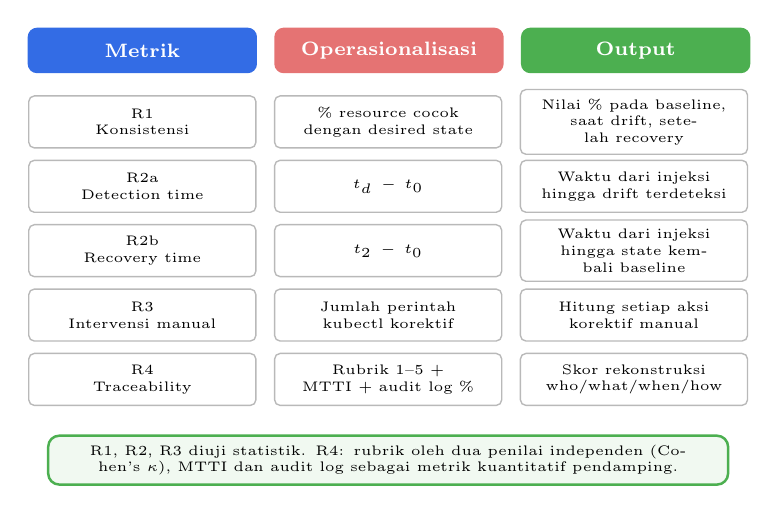
\begin{tikzpicture}[
    node distance=0.14cm and 0.22cm,
    header/.style={rectangle, rounded corners=3pt, draw=#1, fill=#1,
                   text=white, text width=2.65cm, minimum height=0.55cm,
                   align=center, font=\scriptsize\bfseries, line width=0.8pt},
    cell/.style={rectangle, rounded corners=2pt, draw=gray!55, fill=white,
                 text width=2.65cm, minimum height=0.66cm, align=center,
                 line width=0.5pt, font=\tiny},
    note/.style={rectangle, rounded corners=4pt, draw=okgreen, fill=okgreen!8,
                 text width=8.4cm, minimum height=0.60cm, align=center,
                 line width=0.9pt, font=\tiny}
]

\node[header=gitopsblue] (h1) {Metrik};
\node[header=driftred, right=of h1] (h2) {Operasionalisasi};
\node[header=okgreen, right=of h2] (h3) {Output};

\node[cell, below=0.28cm of h1] (m1) {R1\\Konsistensi};
\node[cell, right=of m1] (o1) {\% resource cocok\\dengan desired state};
\node[cell, right=of o1] (u1) {Nilai \% pada baseline,\\saat drift, setelah recovery};

\node[cell, below=of m1] (m2) {R2a\\Detection time};
\node[cell, right=of m2] (o2) {$t_d - t_0$};
\node[cell, right=of o2] (u2) {Waktu dari injeksi\\hingga drift terdeteksi};

\node[cell, below=of m2] (m3) {R2b\\Recovery time};
\node[cell, right=of m3] (o3) {$t_2 - t_0$};
\node[cell, right=of o3] (u3) {Waktu dari injeksi\\hingga state kembali baseline};

\node[cell, below=of m3] (m4) {R3\\Intervensi manual};
\node[cell, right=of m4] (o4) {Jumlah perintah\\kubectl korektif};
\node[cell, right=of o4] (u4) {Hitung setiap aksi\\korektif manual};

\node[cell, below=of m4] (m5) {R4\\Traceability};
\node[cell, right=of m5] (o5) {Rubrik 1--5 +\\MTTI + audit log \%};
\node[cell, right=of o5] (u5) {Skor rekonstruksi\\who/what/when/how};

\node[note, below=0.36cm of o5] (n1)
      {R1, R2, R3 diuji statistik. R4: rubrik oleh dua penilai independen (Cohen's $\kappa$), MTTI dan audit log sebagai metrik kuantitatif pendamping.};

\end{tikzpicture}
\end{document}